\section{Scalability}

\subsection{Boot up times}
One of the selling points of cloud computing is It's scalability. Scalability  is also one of the biggest selling points of unikernel technology. All the literature around unikernels refer to their superior boot up time when compared with containerisation technology. The measurements in figure \ref{fig:boot-up} support that idea. 
\begin{figure}[htpb]
  \centering
  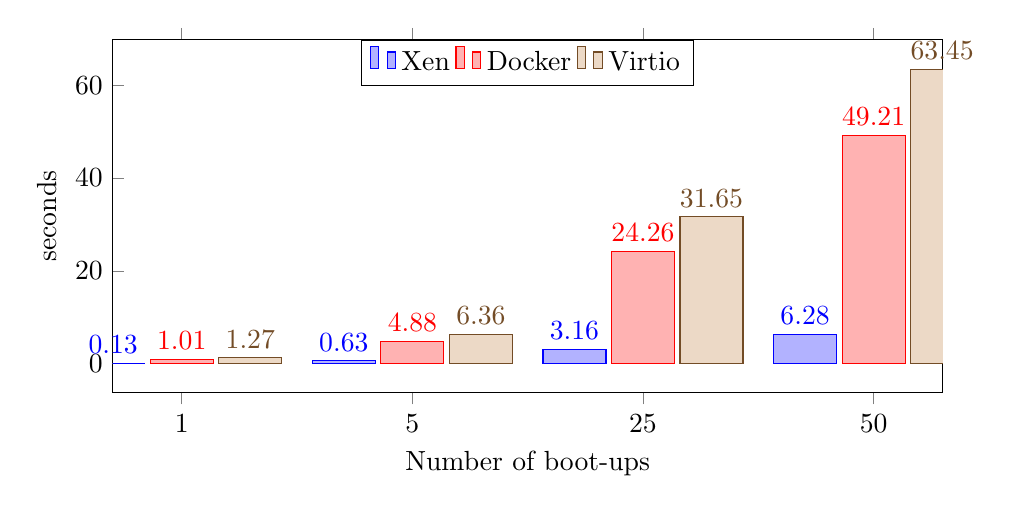
\begin{tikzpicture}
    \begin{axis}[
        ybar,
        bar width=0.8cm,
        width=\textwidth,
        height=.5\textwidth,
        legend style={at={(0.5,1)},
          anchor=north,legend columns=-1},
        ylabel={seconds},
        xlabel={Number of boot-ups},
        symbolic x coords={1,5,25,50},
        xtick=data,
        nodes near coords,
        nodes near coords align={vertical},
        ]
    \addplot coordinates {(1,0.125) (5,0.627) (25,3.157) (50,6.283)};
    \addplot coordinates {(1,1.014) (5,4.881) (25,24.260) (50,49.212)};
    \addplot coordinates {(1,1.268) (5,6.363) (25,31.646) (50,63.446)};
    \legend{Xen,Docker,Virtio}
    \end{axis}
    \end{tikzpicture}
    \caption{Boot-up times}\label{fig:boot-up}
  \end{figure}

The boot up test was conducted by sequentially starting containers and unikernels with a shell script and timing it with \textit{time} command. The docker container was downloaded before, so it's pull time is not part of the thesis. All the test cases use the same program, a hello world, and the docker container only wraps it in ubuntu image. To prevent caching, all images were compiled just before testing. The sizes of the used images can be seen in \ref{tab:sizes}.

The first take from the graph is the boot-up time of Xen hypervisor. It only needs 10-15\% of total boot time required by docker. Starting a single unikernel happends in subsecond and that opens new possibilities of hyper-scalability in the cloud, similar to Jitsu project explained above. We can start boot up new unikernels for on-demand task with virtually no delay to the system or to the user. Another take from the graph is measurements of the virtio\cite{virtio} hypervisor. The reasons for it's inferior boot up times to docker is not known. Virtio is a layer on top of the KVM hypervisor and that might be the case for this delay or it's possible that because of the relation between Xen hypervisor and MirageOS, it's much more compatible to Xen than it is to KVM. It might also be possible because of the virtualisation limitations of the hardware that the test was conducted on.

\subsection{Scaling time}
Another experiment is for measuring scalability of unikernels compared to Docker in Kubernetes. In the following experiments, the setting is the same. There is a 3 node Kubernetes cluster, with a master node, a normal node, and a node connected by virtual kubelet. No pods can be scheduled to run on the master node. The program that is being tested is an infinite loop program that reads data from a file and outputs the value every 2 seconds. The docker container is the same program with ubuntu image wrapped around it. Both nodes have the test image already pulled to their disks. The deployments are already created in Kubernetes. As soon as \textit{scale} command is called, a script counts number of pods with the \textbf{running} status every 0.5 seconds.

\begin{figure}[htpb]
  \centering
  \begin{tikzpicture}
  \begin{axis}[
  axis lines=middle,
  width=\textwidth,
  height=.5\textwidth,
  ymin=0,
  x label style={at={(current axis.right of origin)},anchor=north, below=10mm},
      xlabel=Seconds,
    ylabel=No. of Pods,
    xticklabel style = {rotate=30,anchor=east},
    enlargelimits = false,
    xticklabels from table={scale30.dat}{Time},xtick=data]
  \addplot[orange,thick] table [y=Docker,x=Time]{scale30.dat};
  \addlegendentry{Docker}
  \addplot [green,thick] table [y=Unikernel,x=Time]{scale30.dat};
  \addlegendentry{Unikernel}
  \end{axis}
  \end{tikzpicture}
  \caption{Scaling from 0 to 30 pods}\label{fig:scale-up-30}
  \end{figure}

 \iffalse 
\begin{figure}[htpb]
  \centering
  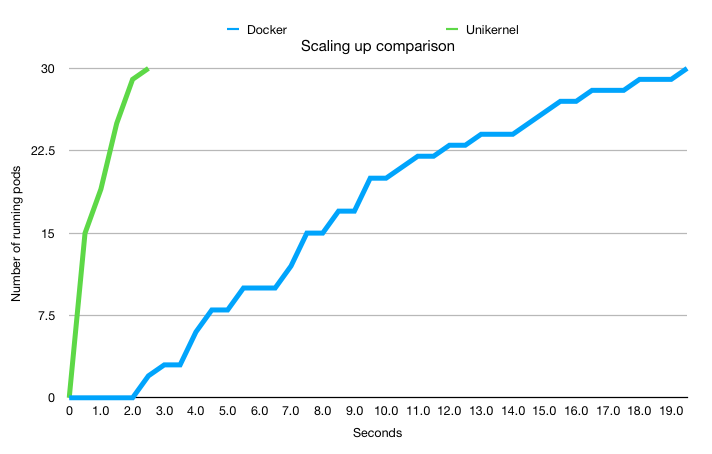
\includegraphics[width=1\textwidth]{figures/scales/scale-up-30.png}
  \caption{Scaling from 0 to 30 pods } \label{fig:scale-up-30}
\end{figure}
\fi

Figure \ref{fig:scale-up-30} shows how fast boot-up time of unikernels in Xen plays a role on their scalability.When given a command to scale from 0 to 30 pods , it only takes 2 seconds for unikernels to boot up. It takes 19 seconds for docker containers. The numbers are smaller than what was measured in boot-up times, because now the programs are being started in parallel instead of sequentially. 


\begin{figure}[htpb]
  \centering
  \begin{tikzpicture}
  \begin{axis}[
  axis lines=middle,
  width=\textwidth,
  height=.5\textwidth,
  ymin=0,
  x label style={at={(current axis.right of origin)},anchor=north, below=10mm},
      xlabel=Seconds,
    ylabel=No. of Pods,
    xticklabel style = {rotate=30,anchor=east},
    enlargelimits = false,
    xticklabels from table={scale50.dat}{Time},xtick=data]
  \addplot[orange,thick] table [y=Docker,x=Time]{scale50.dat};
  \addlegendentry{Docker}
  \addplot[green,thick] table [y=Unikernel,x=Time]{scale50.dat};
  \addlegendentry{Unikernel}
  \end{axis}
  \end{tikzpicture}
  \caption{Scaling from 0 to 50 pods}\label{fig:scale-up-50}
  \end{figure}

  \iffalse
\begin{figure}[htpb]
  \centering
  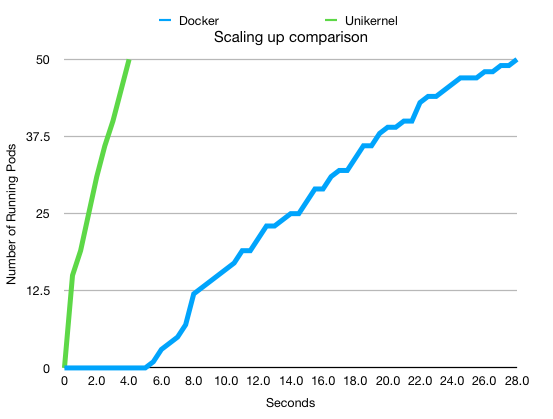
\includegraphics[width=0.7\textwidth]{figures/scales/scale-up-50.png}
  \caption{Scaling from 0 to 50 pods } \label{fig:scale-up-50}
\end{figure}
\fi  
Figure \ref{fig:scale-up-50} draws a similar picture when scaling up from 0 to 50. It takes 4 seconds for all unikernels to start , while docker needs 26 seconds to start them.
\begin{figure}[htpb]
  \centering
  \begin{tikzpicture}
  \begin{axis}[
  axis lines=middle,
  width=\textwidth,
  height=.5\textwidth,
  ymin=0,
  x label style={at={(current axis.right of origin)},anchor=north, below=10mm},
      xlabel=Seconds,
    ylabel=No. of Pods,
    xticklabel style = {rotate=30,anchor=east},
    enlargelimits = false,
    xticklabels from table={scaledown50.dat}{Time},xtick=data]
  \addplot[orange,thick] table [y=Docker,x=Time]{scaledown50.dat};
  \addlegendentry{Docker}
  \addplot [green,thick] table [y=Unikernel,x=Time]{scaledown50.dat};
  \addlegendentry{Unikernel}
  \end{axis}
  \end{tikzpicture}
  \caption{Scaling from 50 to 0 pods}\label{fig:scale-down-50}
  \end{figure}

  \begin{figure}[htpb]
    \centering
    \begin{tikzpicture}
    \begin{axis}[
    axis lines=middle,
    width=\textwidth,
    height=.5\textwidth,
    ymin=0,
    x label style={at={(current axis.right of origin)},anchor=north, below=10mm},
        xlabel=Seconds,
      ylabel=No. of Pods,
      xticklabel style = {rotate=30,anchor=east},
      enlargelimits = false,
      xticklabels from table={scaledown30.dat}{Time},xtick=data]
    \addplot[orange,thick] table [y=Docker,x=Time]{scaledown30.dat};
    \addlegendentry{Docker}
    \addplot [green,thick] table [y=Unikernel,x=Time]{scaledown30.dat};
    \addlegendentry{Unikernel}
    \end{axis}
    \end{tikzpicture}
    \caption{Scaling from 30 to 0 pods}\label{fig:scale-down-30}
    \end{figure}

  \iffalse
\begin{figure}[htpb]
  \centering
  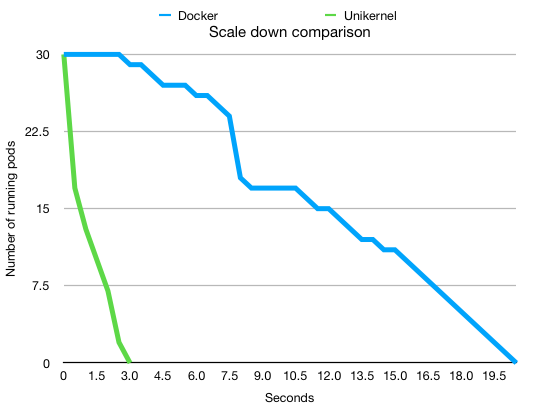
\includegraphics[width=0.7\textwidth]{figures/scales/scale-down-30.png}
  \caption{Scaling from 30 to 0 pods } \label{fig:scale-down-30}
\end{figure}
\fi

\iffalse
\begin{figure}[htpb]
  \centering
  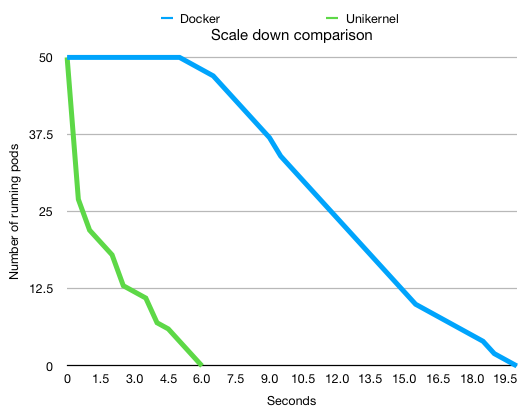
\includegraphics[width=0.7\textwidth]{figures/scales/scale-down-50.png}
  \caption{Scaling from 50 to 0 pods } \label{fig:scale-down-50}
\end{figure}
\fi

Figure \ref{fig:scale-down-30} and \ref{fig:scale-down-50} shows the scaling down time of running pods. The result is similar to scaling up cases. It takes around 5 seconds for unikernels to scale down completely while docker containers need around 20 seconds. 

To measure the performance of scalability of unikernels, we can use the formula proposed by Jindal et al. in \cite{multilayered}. While their formula is for autoscaling systems, It can also be applied here to show the performance difference between unikernels and Docker containers. Since Kubernetes autoscaler can also operate on unikernel resources as it sees them as pods.
\begin{equation*}
  \begin{aligned}
  HL(T_{autoscale})&=\frac{t_d-t_c}{t_b-t_a} \\
  &\textrm{where} \\ 
  T_{autoscale}&=[t_a,t_b] \ \ \textrm{and} \ \ T_{HighLatency}&=[t_c,t_d]
  \end{aligned}
\end{equation*}

We can think of a situation where there is a high request load for 30 seconds, thus \(T_{HighLatency}=[0,30]\). We can use the measurements from figure \ref{fig:scale-up-50}, so we have \(T_{DockerScale}=[0,28]\) and \(T_{UnikernelScale}=[0,4]\). When we put those values in the above equation we get:
\begin{equation*}
  \begin{aligned}
  HL(T_{DockerPerformance})&=\frac{30-0}{28-0}&=\textbf{1.07} \\
  HL(T_{UnikernelPerformance})&=\frac{30-0}{4-0}&=\textbf{7.5} \\
  \end{aligned}
\end{equation*}
For this formula, a result of \textbf{1} means that there was a high latency during the whole scaling interval, which means a higher score is better. The scalability of unikernels has 7 times better performance than docker.


\subsection{Kubernetes reaction time}
There is also another information we can read from the graph, namely how fast Kubernetes distributes information. For example, when we look at Figure \ref{fig:scale-down-50}, and only observe the scaling behaviour of docker containers, we might think that Kubernetes has a delay of 6 seconds when distributing \textit{scale-down} command to other nodes. Same argument would also be true for \textit{scale-up} command when we check other experiments as well. There is a visible delay in all cases where node count stays constant for a couple of seconds at start, then changes rapidly with respect to the command. When we observe the unikernel behavior though, we have a different scenario. The node reacts to command almost instantly, with only half a second delay. This phenomenon is visible in all graphs. We can read that Kubernetes distributes commands instantly around the cluster. This new information makes it plausible to suggest a new argument: "The boot-up times of docker containers is the bottleneck for Kubernetes scalability and different runtimes with better boot up times might help to overcome this problem".


  
